\documentclass[aps,prl,reprint,superscriptaddress,amsmath,amssymb]{revtex4-2}
\usepackage{graphicx,bm,amsthm}
\usepackage[colorlinks=true,citecolor=blue,urlcolor=blue,linkcolor=blue]{hyperref}
\hypersetup{pdftitle={A Common Recovery Transition for Classical and Quantum Information in Random Codes},pdfauthor={Xi Zhao}}
\newtheorem{theorem}{Theorem}
\newtheorem{corollary}{Corollary}
\newcommand{\E}{\mathbb E}
\newcommand{\Prb}{\mathbb P}
\newcommand{\N}{\mathcal N}
\newcommand{\tr}{\operatorname{tr}}
\newcommand{\Pc}{P_{\mathrm c}^{*}}
\newcommand{\Fq}{F_{\mathrm q}^{*}}
\newcommand{\Fs}{\mathcal F}
\begin{document}
\title{A Common Recovery Transition for Classical and Quantum Information in Random Codes}
\author{Xi Zhao}\noaffiliation
\date{October 28, 2026}
\begin{abstract}
Reading classical messages requires less than restoring quantum coherence.
For random codes under Pauli noise, we show that both tasks have the same
critical performance. A finite-size information-spectrum bound sandwiches
optimal entanglement fidelity and classical decoding success for every exact
unitary 2-design. With independent identical errors, it yields a common Gaussian
crossover at positive coding rate, in mean and with high probability.
Clifford codes realize the classical optimum by inverse encoding and basis
measurement followed by classical decoding.
\end{abstract}
\maketitle

Recovering a classical label and recovering a quantum state impose different
demands on an encoding. A phase error can leave every computational-basis
message readable while destroying a superposition. Random quantum encoders
spread both kinds of information over a register. Does allowing the receiver
to discard coherence then postpone the failure of the code?

We compare these two tasks for the \emph{same} random encoder followed by
Pauli noise. The receiver either guesses a uniformly distributed logical-basis
message or restores entanglement with a reference. Each receiver is optimized
with knowledge of the realized encoder. Our result is that, at positive rate,
their optimal performances approach the same Gaussian curve across the coding
transition. Thus the easier classical task has no separate threshold or
second-order rate advantage within this ensemble, even though its finite-size
success probability is larger.

The hashing rate $1-H(\bm p)$ is an established quantum-coding
benchmark~\cite{Bennett,Devetak}. Klesse's random-code argument already yields
truncated-error-spectrum quantum achievability, including a probability
bound over encoders~\cite{Klesse}.
Second-order quantum achievability~\cite{TBR} and finite-size Clifford
analyses~\cite{Darmawan} quantify attainable rates. Haar-code spectra and
coherent information exhibit a hashing transition with a square-root
finite-size window~\cite{Sommers}; approximate quantum Hamming
bounds~\cite{MaTanWright} and stabilizer converses~\cite{StabilizerConverse}
provide complementary constraints. Here a classical decoding converse
matches the quantum achievable profile throughout the critical window.
Together they determine the optimal classical \emph{and} quantum performance
of the same sampled code. The finite-size bracket and its probability bound
require only unitary second moments.

\emph{One encoder, two tasks.}---Let $d=2^n$ and $M=2^k\le d$, with integer
$k\ge1$. Embed the logical space by
$V_0|j\rangle=|j\rangle|0\rangle^{\otimes(n-k)}$ and encode with $V=UV_0$,
where $U$ is drawn from an exact unitary 2-design. Haar and uniform Clifford
encoders are examples~\cite{Dankert}. The same $U$ encodes all messages; the
codewords are orthogonal, not independent random states. A fixed Pauli channel
acts after encoding:
\begin{equation}
\N_p(\rho)=\sum_{P\in\{I,X,Y,Z\}^{\otimes n}}p_PP\rho P^\dagger,
\quad s(P)=-\log_2p_P.
\label{eq:noise}
\end{equation}
The distribution is independent of $U$ and may include correlated errors.
Define $\Fs(t)=\Prb_{P\sim p}[s(P)<t]$. All logarithms are base two.

For $\rho_j=\N_p(V|j\rangle\langle j|V^\dagger)$, the optimal classical
success probability is
\begin{equation}
\Pc(V)=\max_{\{E_j\}}\frac1M\sum_j\tr(E_j\rho_j).
\label{eq:classical}
\end{equation}
Let $|\Phi_M\rangle=M^{-1/2}\sum_j|j\rangle|j\rangle$ and
$\mathcal V(\rho)=V\rho V^\dagger$. The optimal entanglement fidelity is
\begin{equation}
\Fq(V)=\max_{\mathcal D}\langle\Phi_M|
[\mathrm{id}\otimes(\mathcal D\N_p\mathcal V)](\Phi_M)|\Phi_M\rangle,
\label{eq:quantum}
\end{equation}
where $\mathcal D$ is any quantum channel back to the logical space. Fidelity
here is the overlap, not its square root. Both optimizations precede averaging
over $U$. Encoding and decoding are ideal; neither a noise record nor access
to the environment is supplied.

\emph{A common finite-size bracket.}---The following bounds compare the two
optimized tasks without identifying their decoders.
\begin{theorem}
For any distribution in Eq.~\eqref{eq:noise}, any exact unitary 2-design
encoder, and every $a>0$,
\begin{align}
\Fs(n-k-a)-8\,2^{-a}
&\le\E\Fq\le\E\Pc\nonumber\\
&\le\Fs(n-k+2a)+\frac54\,2^{-a}+\frac{2^a}{4M}.
\label{eq:bracket}
\end{align}
Moreover, $\Fq(V)\le\Pc(V)$ for every encoder. With
$F_-=\Fs(n-k-a)$ and $F_+=\Fs(n-k+2a)$, for any $\eta>0$,
\begin{align}
&\Prb_U[\Fq<F_--\eta\ \text{or}\ \Pc>F_++\eta]\nonumber\\
&\hspace{12mm}\le\frac{37\,2^{-a}}{4\eta}+\frac{2^a}{4M\eta}.
\label{eq:highprob}
\end{align}
\end{theorem}

The relevant spectral budget is $n-k$. Likely errors consume physical space
that would otherwise hold logical messages. Quantum recovery is possible for
a sufficiently small likely-error family; the classical converse shows that
abandoning phase information does not recover the spectral mass outside the
same budget. The proof controls overlaps in aggregate and does not replace
error images by independent or exactly orthogonal vectors.

\emph{Proof.}---For a recovered logical channel with Kraus operators $A_\ell$,
\begin{equation}
F_e=\frac1{M^2}\sum_\ell|\tr A_\ell|^2
\le\frac1M\sum_{j,\ell}|(A_\ell)_{jj}|^2\le\Pc.
\label{eq:ordering}
\end{equation}
The middle expression is the success of that recovery followed by a
logical-basis measurement. This proves the pointwise ordering.

For the lower bound, take $\mathcal G=\{s<n-k-a\}$,
$L=|\mathcal G|<d2^{-a}/M$, and define
\begin{equation}
S=\sum_{P\in\mathcal G}PVV^\dagger P^\dagger,\qquad
R_P=V^\dagger P^\dagger S^{-1/2}.
\label{eq:recovery}
\end{equation}
The inverse is on the support of $S$. The $R_P$ obey
$\sum_PR_P^\dagger R_P=\Pi_{\mathrm{supp}S}$; completing them on its kernel
gives a trace-preserving square-root recovery~\cite{BarnumKnill}. For
$v_{jP}=PV|j\rangle$ and $a_{jP}=\langle v_{jP}|S^{-1/2}|v_{jP}\rangle$,
Hayashi--Nagaoka~\cite{HayashiNagaoka} gives
\begin{equation}
1-a_{jP}^2\le4\!\sum_{(i,Q)\ne(j,P)}|\langle v_{jP}|v_{iQ}\rangle|^2
=:4C_{jP}.
\end{equation}
Also $0\le a_{jP}\le1$. Keeping the terms where the actual error matches
the recovery Kraus index in the fidelity sum yields
\begin{align}
F_e&\ge\sum_{P\in\mathcal G}p_P\left(\frac1M\sum_ja_{jP}\right)^2
\ge p(\mathcal G)-8X,\nonumber\\
X&=\sum_{P\in\mathcal G}\frac{p_P}{M}\sum_jC_{jP}.
\label{eq:loss}
\end{align}
The label $P$ in Eq.~\eqref{eq:recovery} is an internal Kraus index, not a
known noise realization. Exact unitary second moments and orthogonality of
the code columns give
\begin{equation}
\E C_{jP}=\frac{(L-1)(dM-1)}{d^2-1}\le\frac{ML}{d},
\end{equation}
so $\E X\le2^{-a}$. This proves the lower bound, including nonuniform error
probabilities. The empty $\mathcal G$ case is trivial.

For the upper bound, every POVM and every $c>0$ satisfy
\begin{equation}
P_{\rm succ}\le\frac{cd}{M}+\frac1M\sum_j\tr(\rho_j-cI)_+.
\end{equation}
Split each output at error probability $c'$ into a head and a tail $B_j$.
The head contributes at most its mass, while
$(\lambda-c)_+\le\lambda^2/(4c)$ bounds the tail. Each code column is a state
2-design, and Pauli orthogonality gives
\begin{equation}
\E\tr B_j^2=\frac{dv_t+m_t^2}{d+1}\le c'+\frac1d,
\end{equation}
where $m_t=\sum_{p_P\le c'}p_P$ and $v_t=\sum_{p_P\le c'}p_P^2\le c'm_t$.
Putting $\gamma=cd$ and $c'=c2^{-a}$ gives
\begin{equation}
\E\Pc\le\frac\gamma M+\frac1{4\gamma}+\frac{2^{-a}}4
+\Fs(n-\log_2\gamma+a).
\label{eq:generalupper}
\end{equation}
Choose $\gamma=M2^{-a}$. The same pointwise constructions control the
positive deviations from $F_-$ and $F_+$; Markov's inequality gives
Eq.~\eqref{eq:highprob}. Full details appear in the Supplemental Material
(SM)~\cite{SM}.

\emph{The shared critical curve.}---For independent identical errors,
$p=\bm p^{\otimes n}$, write $H=\E[-\log_2p_\alpha]$ and
$\sigma^2=\operatorname{Var}[-\log_2p_\alpha]$ for one qubit.
At fixed positive rate $R=k/n$, Eq.~\eqref{eq:bracket} gives exponential
approach to one for $R<1-H$, and exponential decay to zero for
$R>\max(1-H,0)$. These are ensemble-specific coding thresholds.

More precisely, fix $\bm p$ with $0<H<1$ and $\sigma>0$, and let
\begin{equation}
k_n=n(1-H)+\sqrt n\,\sigma z+O(1)
\label{eq:window}
\end{equation}
for fixed $z$. Berry--Esseen~\cite{Feller}, applied to the two CDFs in
Eq.~\eqref{eq:bracket} with $a=2\log_2n$, yields
\begin{equation}
\boxed{\begin{aligned}
\E\Fq&=\Phi(-z)+O\!\left(\frac{\log n}{\sqrt n}\right),\\
\E\Pc&=\Phi(-z)+O\!\left(\frac{\log n}{\sqrt n}\right).
\end{aligned}}
\label{eq:gaussian}
\end{equation}
Here $\Phi$ is the normal CDF. Equation~\eqref{eq:highprob} with
$\eta=n^{-1/2}$ shows that both quantities follow this curve for the same
encoder outside an exceptional set of probability at most
$37/(4n^{3/2})+n^{5/2}/(4M_n)$. The constants are uniform over the choice of
exact 2-design. At a fixed target error $\epsilon$, the classical and quantum
ensemble coding sizes therefore both obey
\begin{equation}
k_\epsilon=n(1-H)+\sqrt n\,\sigma\Phi^{-1}(\epsilon)+O(\log n).
\label{eq:dispersion}
\end{equation}
Errors are respectively $1-\Pc$ and $1-\Fq$. Thus equality extends through
the second-order term, not just the hashing rate. Fixed message dimension,
zero surprisal variance, and the endpoint $H=1$ are outside this Gaussian
statement; Eq.~\eqref{eq:bracket} remains valid there.

\begin{figure*}[t]
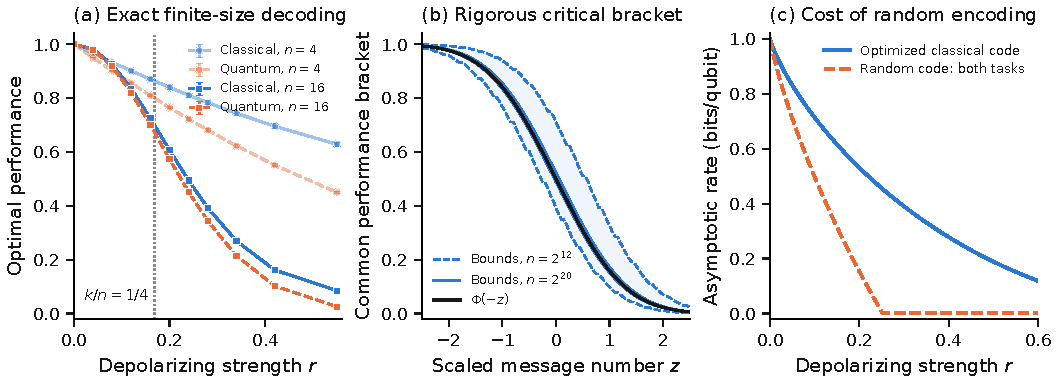
\includegraphics[width=\textwidth]{figures/recovery.pdf}
\caption{Two optimal tasks and one asymptotic transition. (a) Exact classical
success and entanglement fidelity for uniform Clifford encoders with $k/n=1/4$;
64 encoders per size, reused across noise strengths. Markers show encoder
means and one-standard-error bars; lines join points. The vertical line solves
$H(1-3r/4,r/4,r/4,r/4)=3/4$. The finite-size classical advantage is resolved.
(b) Rigorous bounds in Eq.~\eqref{eq:bracket} for $r=0.1$, $a=2\log_2n$,
and $k$ chosen by Eq.~\eqref{eq:window}, compared with $\Phi(-z)$. These are
binomial-CDF evaluations, not large-system decoding simulations.
(c) The common random-code rate $[1-H]_+$ compared with the optimized
classical capacity $1-h_2(r/2)$ of the same depolarizing channel.}
\label{fig:results}
\end{figure*}

\emph{Exact Clifford decoding.}---For a Clifford encoder, conjugating a
physical error through $U^\dagger$ produces logical Pauli labels $(x,z)$ and
an auxiliary bit-flip syndrome $s$. Let $w(s,x,z)$ include the probability of
all physical errors with these labels. Auxiliary phase errors are summed.
Orthogonal syndrome sectors reduce optimal quantum recovery to correction of
the most likely logical Pauli~\cite{StabilizerConverse}, while phase labels
are irrelevant to a classical basis message. Consequently,
\begin{align}
\Fq&=\sum_s\max_{x,z}w(s,x,z),\nonumber\\
\Pc&=\sum_s\max_x\sum_z w(s,x,z).
\label{eq:clifford}
\end{align}
The classical outputs commute. Inverse Clifford encoding, computational-basis
measurement, and classical maximum-likelihood processing attain $\Pc$.
The processing is not guaranteed to be efficient. Equation~\eqref{eq:clifford}
also makes the finite-size advantage transparent: classical decoding can
combine errors that differ only in their logical phase. The theorem states
that this advantage does not survive at leading order inside the regular
critical window.

We evaluate Eq.~\eqref{eq:clifford} for $n=4,8,12,16$, using an exact binary
Fourier sum over syndrome and logical labels. No independent-vector or
random-matrix replacement is made. Figure~\ref{fig:results}(a) shows the
smallest and largest sizes. Independent direct Pauli enumeration and
primal--dual semidefinite optimization at $n\le3$ check both scores and the
explicit recovery construction; methods, all sizes, seeds, and raw encoder
values accompany the SM. The modest simulated sizes illustrate finite-size
behavior; the shared asymptotic curve follows from the proof and its spectral
bounds [Fig.~\ref{fig:results}(b)].

\emph{What random encoding costs.}---The common rate is a property of random
quantum encoders, not an equality of classical and quantum channel capacities.
For $\N_r(\rho)=(1-r)\rho+rI/2$, classical product-state coding achieves the
capacity $1-h_2(r/2)$~\cite{King}. At $r=0.1$ it is $0.714$ bits per qubit,
whereas the common random-code rate is $0.497$. The latter vanishes at
$r_c=0.252386\ldots$, where the optimized classical capacity is still
$0.453$ [Fig.~\ref{fig:results}(c)]. Thus the noise continues to support
classical communication after these random encodings lose every positive
rate. The receiver's permission to discard coherence does not recover the
encoding advantage of a code designed specifically for classical messages.

Random-state contraction~\cite{Ibarrondo} and coherent
information~\cite{Sommers} probe related aspects of noisy encodings.
Liu \emph{et al.} also bound accessible information for a full state-2-design
alphabet~\cite{Liu}. Here the alphabet is the $M$ orthogonal columns at
fixed, known $U$: the receiver optimizes separately for that alphabet before
we average over $U$. A classical converse for this conditional codebook
matches quantum achievability, explaining the common recovery curve.
Extending this result to approximate designs and noise accumulated during
encoding would connect it to finite-depth devices.

\emph{Acknowledgments.}---Generative AI was used substantively for problem
selection, derivations, literature searches, code, figures, and manuscript
preparation, including independent model-assisted review. Tools included
Claude Code with Claude Opus 5.5 and the session model identified as
\texttt{mythos-magpie-2161436569}; an earlier external GPT review had an
unrecorded model version. The author is responsible for the submitted work.
The new recovery theorem has not been formalized in Lean; an earlier
conditional two-state formalization is retained separately.

\emph{Data availability.}---Source, raw encoder samples, numerical verification
records, and figure data are supplied with this manuscript. No public archive
identifier has yet been assigned.

\begin{thebibliography}{99}
\bibitem{Bennett} C. H. Bennett, D. P. DiVincenzo, J. A. Smolin, and W. K. Wootters, Mixed-state entanglement and quantum error correction, Phys. Rev. A \textbf{54}, 3824 (1996).
\bibitem{Devetak} I. Devetak, The private classical capacity and quantum capacity of a quantum channel, IEEE Trans. Inf. Theory \textbf{51}, 44 (2005).
\bibitem{Klesse} R. Klesse, Approximate quantum error correction, random codes, and quantum channel capacity, Phys. Rev. A \textbf{75}, 062315 (2007).
\bibitem{TBR} M. Tomamichel, M. Berta, and J. M. Renes, Quantum coding with finite resources, Nat. Commun. \textbf{7}, 11419 (2016).
\bibitem{Darmawan} A. S. Darmawan, Y. Nakata, S. Tamiya, and H. Yamasaki, Low-depth random Clifford circuits for quantum coding against Pauli noise using a tensor-network decoder, Phys. Rev. Research \textbf{6}, 023055 (2024).
\bibitem{Sommers} G. M. Sommers, J. A. Jacoby, Z. Weinstein, D. A. Huse, and S. Gopalakrishnan, Spectral properties and coding transitions of Haar-random quantum codes, PRX Quantum \textbf{7}, 020328 (2026).
\bibitem{MaTanWright} F. Ma, X. Tan, and J. Wright, Haar random codes attain the quantum Hamming bound, approximately, \href{https://arxiv.org/abs/2510.07158}{arXiv:2510.07158} (2025).
\bibitem{StabilizerConverse} M. Tomamichel, A strong converse for stabilizer codes over Pauli channels via the blowing-up lemma, \href{https://arxiv.org/abs/2607.23450}{arXiv:2607.23450} (2026).
\bibitem{Dankert} C. Dankert, R. Cleve, J. Emerson, and E. Livine, Exact and approximate unitary 2-designs and their application to fidelity estimation, Phys. Rev. A \textbf{80}, 012304 (2009).
\bibitem{BarnumKnill} H. Barnum and E. Knill, Reversing quantum dynamics with near-optimal quantum and classical fidelity, J. Math. Phys. \textbf{43}, 2097 (2002).
\bibitem{HayashiNagaoka} M. Hayashi and H. Nagaoka, General formulas for capacity of classical-quantum channels, IEEE Trans. Inf. Theory \textbf{49}, 1753 (2003).
\bibitem{SM} See Supplemental Material for the full recovery proof, probability bounds, second-order inversion, Clifford optimality, and numerical methods.
\bibitem{Feller} W. Feller, \emph{An Introduction to Probability Theory and Its Applications}, Vol.~II, 2nd ed. (Wiley, New York, 1971), Sec.~XVI.5.
\bibitem{King} C. King, The capacity of the quantum depolarizing channel, IEEE Trans. Inf. Theory \textbf{49}, 221 (2003).
\bibitem{Ibarrondo} R. Ibarrondo and D. Stilck Fran\c{c}a, Average contraction coefficients of quantum channels, \href{https://arxiv.org/abs/2508.08214}{arXiv:2508.08214} (2025).
\bibitem{Liu} G. Liu, C. Qin, Z. Xu, X. Ma, and Z.-W. Liu, Can scrambling protect quantum state distinguishability under noise?, \href{https://arxiv.org/abs/2606.02122}{arXiv:2606.02122} (2026).
\end{thebibliography}
\end{document}
